\documentclass{article}

\usepackage{graphicx}
\usepackage{tikz}
\usepackage{tikzsymbols}
\usetikzlibrary{calc,patterns,shapes.geometric}
\pagestyle{empty}
\usepackage[margin=0pt]{geometry}
\geometry{papersize={14in,12in}}

\def\centerarc[#1](#2)(#3:#4:#5){\draw[#1] ($(#2)+({#5*cos(#3)},{#5*sin(#3)})$) arc (#3:#4:#5);}

\begin{document}
	\begin{figure}
		\centering
		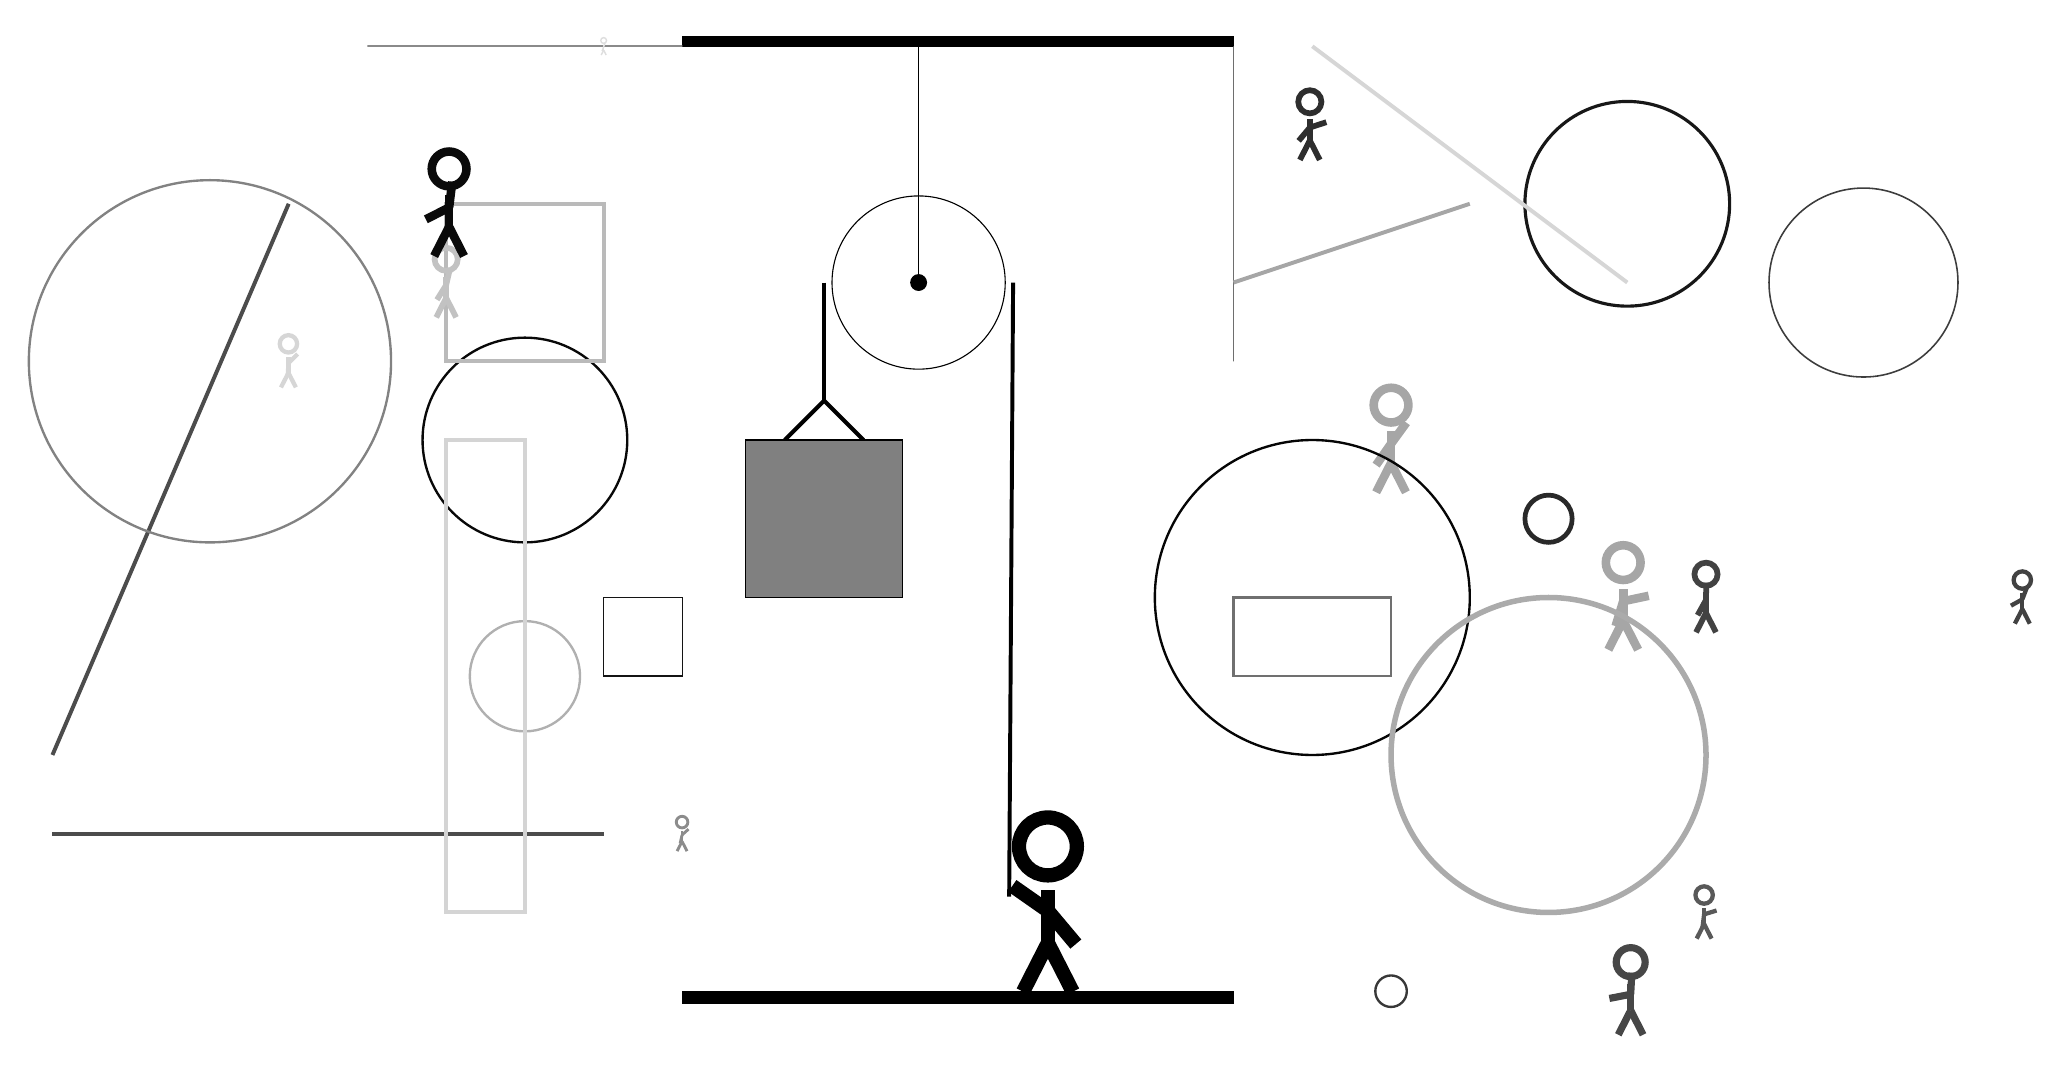
\begin{tikzpicture}
			%%%%% START %%%%%
			
			\draw[fill=black] (-2, 9) rectangle (5, 9.125);
			
			\draw (1, 6) circle (1.1);
			\draw[fill=black] (1, 6) circle (0.1);
			\draw (1, 9) -- (1, 6);
			
			\draw[line width=0.5mm] (-0.7, 4.0) -- (-0.2, 4.5) -- (0.3, 4.0);
			\draw[fill=black!50] (-1.2, 4.0) rectangle (0.8, 2.0);
			
			\draw[line width=0.5mm] (-0.2, 6) -- (-0.2, 4.5);
			\centerarc[line width=0.5mm](1, 6)(0:180:1.2000000000000002);
			\draw[line width=0.5mm](2.2, 6) -- (2.15, -1.8);
			
			\draw[line width=0.2mm, color=black!57] (5, 9) rectangle (5, 5);
			
			\draw [line width=0.3mm, color=black!97](-4, 4) circle (1.3);
			\node[line width=0.6mm, color=black!82] at (6, 8) {\Strichmaxerl[4][50][18]};
			\draw[line width=0.2mm, color=black!92] (-2, 2) rectangle (-3, 1);
			\draw [line width=0.2mm, color=black!76](13, 6) circle (1.2);
			\draw[line width=0.5mm, color=black!27] (-3, 5) rectangle (-5, 7);
			\node[line width=0.4mm, color=black!65] at (11, -2) {\Strichmaxerl[3][83][17]};
			\node[line width=0.5mm, color=black!45] at (-2, -1) {\Strichmaxerl[2][77][42]};
			\draw [line width=0.4mm, color=black!91](10, 7) circle (1.3);
			
			\draw[line width=0.5mm, color=black!70](-7, 7) -- (-10, 0);
			\draw [line width=0.3mm, color=black!31](-4, 1) circle (0.7);
			\draw[line width=0.3mm, color=black!46] (-2, 9) rectangle (-6, 9);
			\node[line width=0.6mm, color=black!13] at (-3, 9) {\Strichmaxerl[1][69][72]};
			
			\draw [line width=0.3mm, color=black!49](-8, 5) circle (2.3);
			\draw [line width=0.3mm, color=black!78](7, -3) circle (0.2);
			\node[line width=0.6mm, color=black!72] at (10, -3) {\Strichmaxerl[5][11][87]};
			
			\node[line width=0.3mm, color=black!35] at (7, 4) {\Strichmaxerl[6][55][54]};
			\draw[line width=0.5mm, color=black!70](-3, -1) -- (-10, -1);
			\node[line width=0.6mm, color=black!24] at (-5, 6) {\Strichmaxerl[4][58][77]};
			\node[line width=0.7mm, color=black!35] at (10, 2) {\Strichmaxerl[6][73][12]};
			\node[line width=0.4mm, color=black!16] at (-7, 5) {\Strichmaxerl[3][87][45]};
			\draw[line width=0.5mm, color=black!16](6, 9) -- (10, 6);
			\node[line width=0.6mm, color=black!74] at (15, 2) {\Strichmaxerl[3][29][69]};
			\node[line width=0.6mm, color=black!74] at (11, 2) {\Strichmaxerl[4][61][89]};
			\draw[line width=0.5mm, color=black!17] (-4, 4) rectangle (-5, -2);
			
			\draw [line width=0.3mm, color=black!98](6, 2) circle (2.0);
			
			\node[line width=0.5mm, color=black!96] at (-5, 7) {\Strichmaxerl[6][27][83]};
			\draw [line width=0.6mm, color=black!84](9, 3) circle (0.3);
			
			\draw [line width=0.7mm, color=black!33](9, 0) circle (2.0);
			\draw[line width=0.3mm, color=black!56] (5, 2) rectangle (7, 1);
			\draw[line width=0.5mm, color=black!35](8, 7) -- (5, 6);
			
			\node at (2.6, -1.9) {\Strichmaxerl[10][-35][-50]};
			
			\draw[fill=black] (-2, -3) rectangle (5, -3.15);
			
			%%%%% END %%%%%
		\end{tikzpicture}
	\end{figure}	
\end{document}